\chapter{The case of WASP-18b}\label{chap:wasp18}

\section{The system}
WASP-18b is a transiting hot Jupiter discovered by \cite{Hellier2009} within the WASP-South transit survey \citep{Pollacco2006}. It is an extremely close-in planet orbiting a F6 type star with a period of 0.94 days. Regarding its physical properties, WASP-18b is about ten times more massive than Jupiter with approximately the same size ($M_{P}=10.3\,{\rm M_{Jupiter}}$, $R_{P}=1.1\,{\rm R_{Jupiter}}$). Even though a rapid orbital decay was predicted theoretically \citep{Hellier2009}, it is not observed yet \citep{Wilkins2017} and new theoretical models proposed a variation of less than 4 seconds in the transit time over a 20-yr baseline \citep{CollierCameron2018}. 


\begin{figure}
\centering
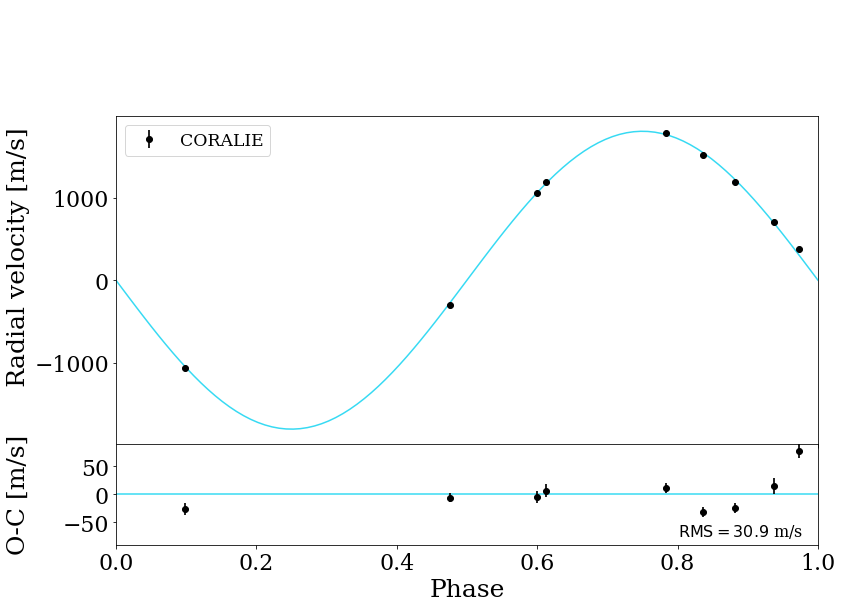
\includegraphics[width=0.7\columnwidth]{imagenes/W18_RV.png}
\caption{Radial velocity fit of WASP-18 }
\label{rv_wasp18}
\end{figure}

\begin{figure}
\centering
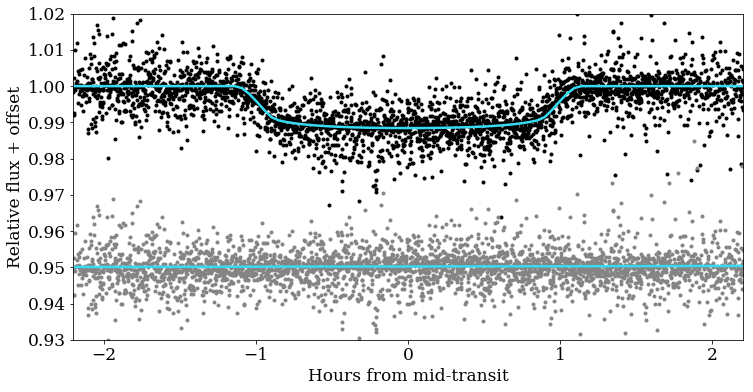
\includegraphics[width=0.7\columnwidth]{imagenes/W18_PHASE.png}
\caption{Phase photometry of WASP-18 }
\label{phase_wasp18}
\end{figure}

\begin{figure}
\centering
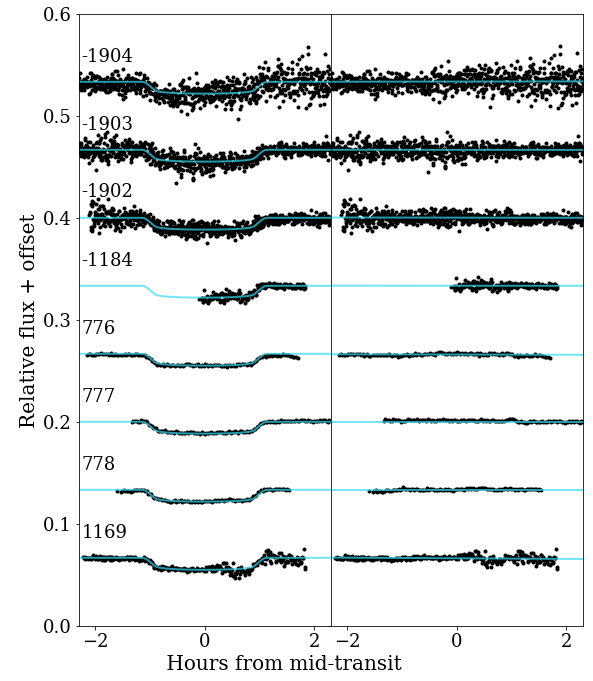
\includegraphics[width=1.0\columnwidth]{imagenes/W18_LC.png}
\caption{Light curves of WASP-18 }
\label{lc_wasp18}
\end{figure}



\section{Observations and Data Reduction}

\begin{table*}
\caption{Log of Observations}             
\label{log_table}      
\centering          
\begin{tabular}{cccccccc}
\hline\hline       
 Date & Epoch\footnotemark{a} & Telescope & Filter & Total exposures & Exposure time\footnotemark{b} & RMS\footnotemark{c} \\
 (UTC) &       &           &       &                   & (seconds) & (mmag)\\
\hline  
 2009 Oct 28 &-1904 & SMARTS 1 m & $I$ & 1412 & 1.5 & 8.49  \\
 2009 Oct 29 & -1903 & SMARTS 1 m & $I$ & 1435 & 2 & 5.67 \\
2009 Oct 30 & -1902 & SMARTS 1 m & $I$ & 1198 & 2  & 4.50 \\
 2011 Sep 06 & -1184 & SMARTS 1 m & $I$ & 203 & 15 & 2.40 \\
2016 Sep 24\footnotemark{d} & 776 & Danish 1.54 m & $I$ & 138 & 90 & 1.05  \\
2016 Sep 25\footnotemark{d} & 777 &Danish 1.54 m & $I$ & 159 & 90  & 0.96  \\
2016 Sep 26\footnotemark{d} & 778 & Danish 1.54 m & $I$ & 113 & 90 & 0.87  \\ \smallskip
2017 Sep 29\footnotemark{d} & 1169 & Danish 1.54 m & $R$ & 330 & 30 & 2.53 \\
\hline                  
\end{tabular}
\footnotetext{a}{The epoch 0 is $T_{0}$ in Tables , for WASP-18b, WASP-19b and WASP-77Ab, respectively.}
\footnotetext{b}{For the variable exposure times, we consider the average during the night.}
\footnotetext{c}{The RMS values were computed from the best fitted model of each light curve.}
\footnotetext{d}{Light curves obtained with only one reference star.}
\end{table*}


\section{Transit Parameters and Physical Properties}\label{transitparams}

The resulting parameters from the global fit of WASP-18 in comparison the with results of the discovery paper \cite{Hellier2009} and the most recent analysis with TESS data \citep{Shporer2018}, are listed in Table~\ref{wasp18}. While in \cite{Hellier2009} the analysis was performed combining photometry and RV data, in \cite{Shporer2018} only photometric data was used. 

%Stellar params
As the stellar spectroscopic priors were taken from the discovery paper \cite{Hellier2009}, our results for the stellar mass $M_*$ and radius $R_*$ are in good agreement with theirs, as expected, as well as the rest of the stellar parameters. \cite{Shporer2018} do not present results of stellar parameters.

%Primary transit params
In the case of the primary transit parameters, the greatest difference is found in the radius of the planet in stellar radii $R_{p}/R_{*}$. Our reported $R_{p}/R_{*}$ is $7.8\sigma$ and $4.4\sigma$ larger that the reported by \cite{Hellier2009} on the discovery paper and the recent result from \cite{Shporer2018}, respectively.  Our transit duration $T_{14}$ is also $3.4\sigma$ larger than the value from \cite{Hellier2009}.

% RV params
For the radial velocity parameters, the RV semi-amplitude derived from our analysis is consistent with the value of \cite{Hellier2009}, as the same data was used. 

% Derived params
Finally, the derived parameters of the system are, in general, in good agreement with the values from \cite{Hellier2009} and \cite{Shporer2018}. 



\begin{landscape}
\begin{longtable}{llccc}
\caption{System parameter of WASP-18}
\label{wasp18}
\centering
\tabularnewline
\hline 
Parameter & Units & This work & \cite{Hellier2009} & \cite{Shporer2018} \\
\hline
\smallskip\\\multicolumn{2}{l}{Stellar Parameters:}&\smallskip\\
~~~~$M_*$  &Mass (\(M_\odot\))  &$1.294^{+0.063}_{-0.061}$ & $1.25\pm0.13$ &  \\
~~~~$R_*$  &Radius (\(R_\odot\))  &$1.319^{+0.061}_{-0.062}$ &$1.26^{+0.067}_{-0.054}$ & \\
~~~~$L_*$  &Luminosity (\(L_\odot\))  &$2.68^{+0.28}_{-0.26}$ & &\\
~~~~$\rho_*$  &Density (cgs)  &$0.795^{+0.11}_{-0.089}$ & $ 0.707^{+0.056}_{-0.096}$&\\
~~~~$\log{g}$  & Surface gravity (cgs)  &$4.310^{+0.036}_{-0.033}$ &$4.367^{+0.028}_{-0.042}$ & \\
~~~~$T_{\rm eff}$  &Effective Temperature (K)  &$6432\pm48$ & $6400\pm100$& \\
~~~~$[{\rm Fe/H}]$  &Metallicity   &$0.107\pm0.080$ & $0.00\pm0.09$ & \\
~~~~$Age$  &Age (Gyr)  &$1.57^{+1.4}_{-0.94}$ & $0.5-1.5$ & \\
%~~~~$d$  &Distance (pc)  &$122.2^{+9.9}_{-8.2}$ & $100\pm10$ & \\

\smallskip\\\multicolumn{2}{l}{Planetary Parameters:}&\smallskip\\
~~~~$R_P$  &Radius (\rj)  &$1.310\pm0.071$ & $1.106^{+0.072}_{-0.054}$& $1.192\pm0.038$\\
~~~~$M_P$  &Mass (\mj)  &$10.48^{+0.42}_{-0.40}$ & $10.30\pm0.69$ & \\
~~~~$P$  &Period (days)  &$0.94145236\pm(49)$ & $0.94145299\pm(87)$& $0.9414576^{(+34)}_{(-35)}$ \\
~~~~$e$  &Eccentricity   &$0.0061^{+0.0089}_{-0.0044}$ & &\\
~~~~$a$  &Semi-major axis (AU)  &$0.02054^{+0.00033}_{-0.00032}$ & $0.02045\pm0.00067$&\\
~~~~$\omega_*$  &Argument of Periastron (Degrees)  &$-100^{+110}_{-120}$ &  &\\
~~~~$\rho_P$  &Density (cgs)  &$5.79^{+0.97}_{-0.78}$& $7.73^{+0.78}_{-1.27}$\footnotemark{b} & \\
~~~~$logg_P$  &Surface gravity   &$4.180^{+0.044}_{-0.041}$ & $4.289^{+0.027}_{-0.050}$ &\\
~~~~$T_{eq}$  &Equilibrium temperature (K)  &$2485^{+53}_{-56}$ & $2384^{+58}_{-30}$ & \\
~~~~$\Theta$  &Safronov Number   &$0.254^{+0.015}_{-0.014}$ & &\\
~~~~$\fave$  &Incident Flux (\fluxcgs)  &$8.66^{+0.77}_{-0.75}$ & & \\

\smallskip\\\multicolumn{2}{l}{Primary Transit Parameters:}&\smallskip\\
~~~~$T_0$  &Transit time (\bjdtdb)  &$2456740.80560\pm(19)$ & $2454221.48163\pm(38)$ & $2458361.048072^{(+34)}_{(-35)}$\\
~~~~$i$  &Inclination (Degrees)  &$83.5^{+2.0}_{-1.6}$ & $86.0\pm2.5$ & $84.31^{+0.40}_{-0.37}$\\
~~~~$R_P/R_*$  &Radius of planet in stellar radii   &$0.1021\pm0.0011$ &  $0.0935\pm0.0011$ & $0.09721^{+0.00016}_{-0.00017}$\\
~~~~$a/R_*$  &Semi-major axis in stellar radii   &$3.35^{+0.15}_{-0.13}$ & & $3.523^{+0.028}_{-0.027}$\\
~~~~$b$  &Impact parameter   &$0.433^{+0.07}_{-0.10}$ & $0.25\pm0.15$ & $0.349^{+0.020}_{-0.022}$\\
~~~~$\delta$  &Transit depth (fraction)  &$0.01041\pm0.00022$ & & $0.009449^{+0.000032}_{-0.000032}$\\
~~~~$u_{1,I}$  &linear LD coeff., I band  &$0.207\pm0.019$ & &\\
~~~~$u_{2,I}$  &quadratic LD coeff., I band  &$0.313\pm0.019$& &\\
~~~~$u_{1,R}$  &linear LD coeff., R band  & $0.257\pm0.045$ & &\\
~~~~$u_{2,R}$  &quadratic LD coeff., R band  &$0.309\pm0.048$ & &\\
~~~~$T_{14}$  &Total transit duration (days)  &$0.0931^{+0.0011}_{-0.0010}$ & $0.08932\pm0.00068$ &\\
~~~~$P_T$  &A priori non-grazing transit prob   &$0.268^{+0.011}_{-0.012}$ & &\\
~~~~$P_{T,G}$  &A priori transit prob   &$0.328^{+0.014}_{-0.015}$ & &\\
~~~~$\tau$  &Ingress/egress transit duration (days)  &$0.0107\pm0.0010$ & &\\

\smallskip\\\multicolumn{2}{l}{RV Parameters:}&\smallskip\\
~~~~$ecos{\omega_*}$  &   &$-0.0004^{+0.0038}_{-0.0045}$ & &\\
~~~~$esin{\omega_*}$  &   &$-0.0008^{+0.0056}_{-0.0092}$ & &\\
~~~~$K$  &RV semi-amplitude (m/s)  &$1807^{+34}_{-36}$ & $1818.3\pm8.0$ &\\
~~~~$M_P\sin i$  &Minimum mass (\mj)  &$10.40\pm0.40$ & &\\
\smallskip\\\multicolumn{2}{l}{Secondary Eclipse Parameters:}&\smallskip\\
~~~~$T_S$  &Time of eclipse (\bjdtdb)  &$2457657.3076^{+0.0023}_{-0.0027}$ & &\\
~~~~$b_S$  &Eclipse impact parameter   &$0.431^{+0.070}_{-0.100}$ & &\\
~~~~$\tau_S$  &Ingress/egress eclipse duration (days)  &$0.0106^{+0.0011}_{-0.0010}$ & &\\
~~~~$T_{S,14}$  &Total eclipse duration (days)  &$0.0929\pm0.0017$ & &\\
~~~~$P_S$  &A priori non-grazing eclipse prob   &$0.269^{+0.010}_{-0.011}$ & &\\
~~~~$P_{S,G}$  &A priori eclipse prob   &$0.330^{+0.013}_{-0.014}$ & &\\
\hline 
\end{longtable}
\end{landscape}
%\tablefoot{
%\tablefoottext{a}{Value converted to cgs units multiplying by the Sun density $\rho_{\odot}=1.408\,$cgs.}
%\tablefoottext{b}{Value converted to cgs units multiplying by the Jupiter density $\rho_{J}=1.33\,$cgs.}
%\tablefoottext{c}{Values enclosed in parentheses correspond to the uncertainties of the last digits of the nominal value.}}




\section{Transit Timing Variations}\label{ttvsection}

%\begin{figure*}
%\vspace{0cm}\hspace{0cm}
%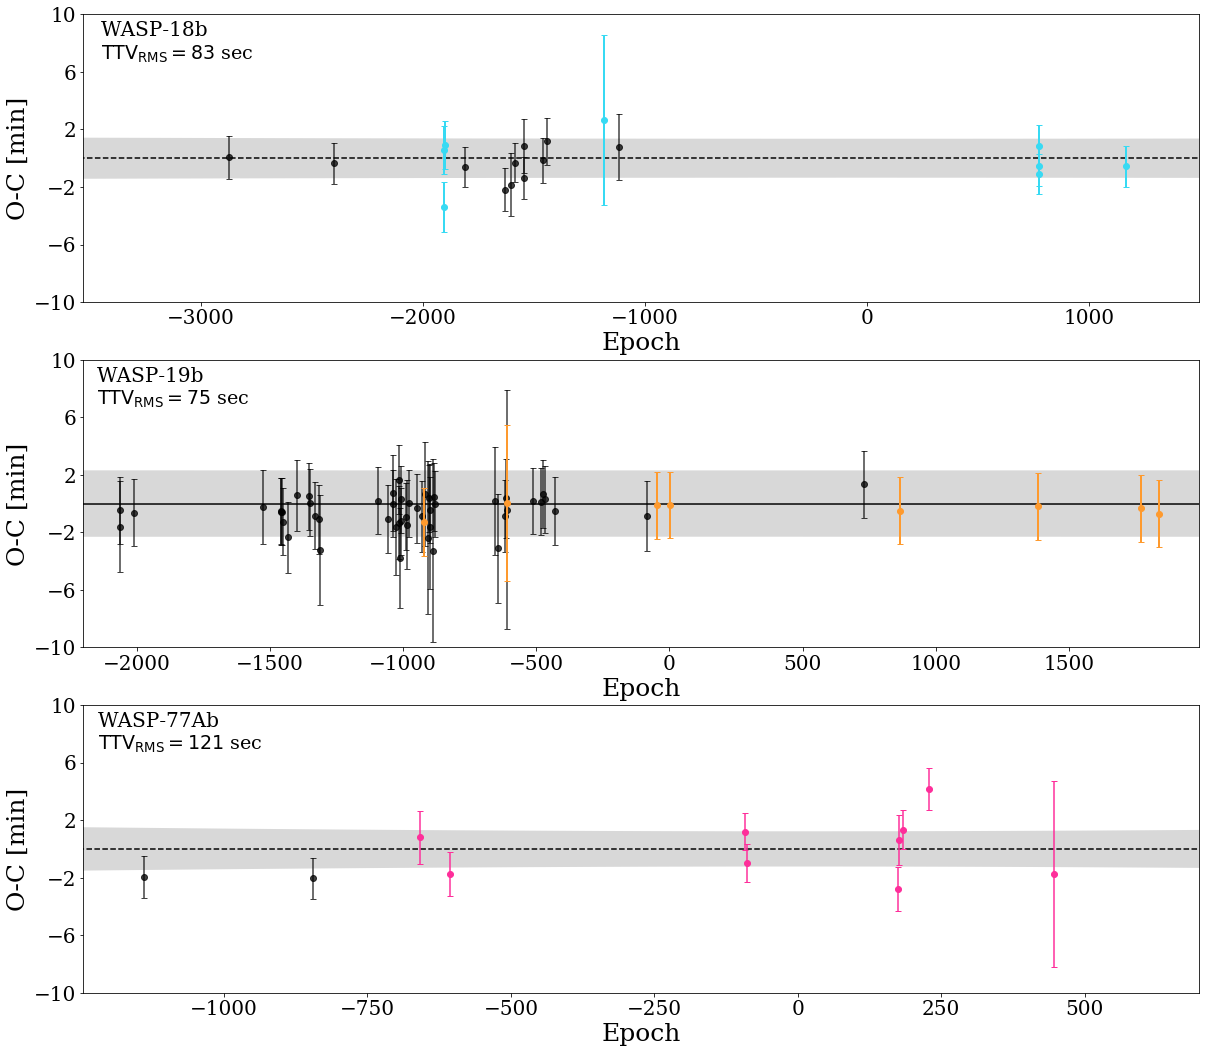
\includegraphics[width=1.0\textwidth]{TTVs.png}
%\centering
%\caption{Observed minus calculated mid-transit times (TTV) for WASP-18b (top), WASP-19b (center) and WASP-77Ab (bottom). The dashed black line corresponds to the proposed linear ephemeris, i.e. zero deviation from the predicted transit time (See Section \ref{ttvsection}) computed from our refined orbital period. For that, we considered 19, 59 and 11 transit times of WASP-18b, WASP-19b, and WASP-77Ab, respectively. The grey area corresponds to the error propagation at $1\sigma$, where the quadratic trend looks almost horizontal. The points in color are the TTV from the newly light curves of the TraMoS project (WASP-18b: light blue, WASP-19b: orange, WASP-77Ab: pink) and the black points in the three panels are TTVs measured from previous published transit times. The RMS scatter from the linear ephemeris are 83 seconds for WASP-18b; 75 seconds for WASP-19b, and 121 seconds for WASP-77Ab.}
%\label{ttv}
%\end{figure*}

For this system, the proposed linear ephemeris equation is:

\begin{equation} \label{eq1_w18}
T_{\rm C}(E)=2456926.27460\pm(94)+E \cdot 0.941452232\pm(89)
\end{equation}

The orbital period $P$ in Eq.~\ref{eq1_w18} is in complete agreement with the value computed only with the TraMoS light curves in Table~\ref{wasp18}.

Table~\ref{times_wasp18} lists the TTV of our transit times and also, of data from previous works \citep{Triaud2010,Hellier2009,Maxted2013b} of WASP-18b. 

The top panel of Figure... is the linear plot of TTV versus epoch for this planet. The deviations of the transit times from the linear ephemeris has an RMS of 83 seconds. The greater deviations come from the transit time of the epochs $-1904$ and $-1184$, which are over the linear ephemeris by $2.5\sigma$ and $1.9\sigma$, respectively. If those values are removed, the RMS decreases to 61 seconds. Considering all the transit times in Table~\ref{times_wasp18} without the epochs $-1904$ and $-1184$, all the TTVs lie within $1.6\sigma$ in the linear fit. 

The epoch $-1184$ has the greatest error in our sample because it is not a complete transit.

When testing the goodness of the linear fit, $\chi^{2}_{red} =0.56$, while for a second degree polynomial is $\chi^{2}_{red}=0.48$, therefore an orbital decay can be discarded in agreement with theoretical estimations \citep{CollierCameron2018}.  


\begin{table}[H]
%\tablewidth{0pt}
\centering
\caption{Transit mid-times for WASP-18b}
\label{times_wasp18}
\begin{tabular}{cccc}
\hline \hline
Epoch & Transit mid-time & TTV & References\\
      & (${\rm BJD_{TDB}}$) & (min) & \\
\hline 
-2873 & $2454221.48238$ & $0.1\pm1.5$ & 1\\
-2402 & $2454664.9061$ & $-0.4\pm1.4$ & 2 \\
-1904 & $2455133.7472$ & $-3.4\pm1.7$ & This work \\
-1903 & $2455134.6914$ & $0.6\pm1.7$ & This work \\
-1902 & $2455135.6331$  & $0.9\pm1.7$  & This work \\
-1811 & $2455221.3042$ & $-0.6\pm1.4$  & 3\\
-1629 & $2455392.6474$ & $-2.2\pm1.5$& 3 \\
-1601 & $2455419.0083$ & $-1.8\pm2.2$& 3\\
-1587 & $2455432.1897$ & $-0.3\pm1.4$ & 3\\
-1546 & $2455470.7885$ & $-1.4\pm1.4$ & 3\\
-1543 & $2455473.6144$ & $0.9\pm1.9$& 3\\
-1457 & $2455554.5786$ & $-0.2\pm1.5$&3 \\
-1440 & $2455570.5842$ & $1.2\pm1.6$& 3\\
-1184 & $2455811.5970$ &  $2.7\pm5.9$ & This work  \\
-1115 & $2455876.5559$ & $0.8\pm2.3$ & 3 \\ 
776 & $2457656.84078$ & $-1.1\pm1.4$ & This work  \\
777 & $2457657.78359$   & $0.9\pm1.4$ & This work\\
778 & $2457658.72404$ & $-0.6\pm1.4$ & This work \\
1169 & $2458026.83186$ & $-0.6\pm1.5$ & This work  \\
\hline
\end{tabular}
%\tablebib{(1)~\citet{Hellier2009};
%(2) \citet{Triaud2010}; (3) \citet{Maxted2013}.}
\end{table} 

\section{Limits on an additional perturber}

For the WASP-18b system we find a large region of instability when compared to the other two systems with the boundaries at the 1:2 interior and 2:1 exterior mean-motion resonance. By over-plotting the RMS scatter of mid-transit times ($\rm TTV_{\rm RMS}$) for a certain value, we find that the TTVs are relatively more sensitive at orbital architectures involving mean-motion resonances confirming the results by \citet{Agol2005} and \citet{Holman2005}. %This also applies to WASP-19 and WASP-77A.

As shown in Figure~\ref{megno_wasp18}, we find that a perturbing body of mass (upper limit) around $7-500~M_{\oplus}$ will produce an RMS of $83\,{\rm s}$ when located in the $P_2/P_1=$ 7:3, 5:2, 3:1, 17:5 and 4:1 exterior resonance. For the 1:3 interior resonance, a perturber mass (upper limit) as small as $1.9~M_{\oplus}$ could also cause a RMS mid-transit time scatter of $83\,{\rm s}$.

\begin{figure}[H]
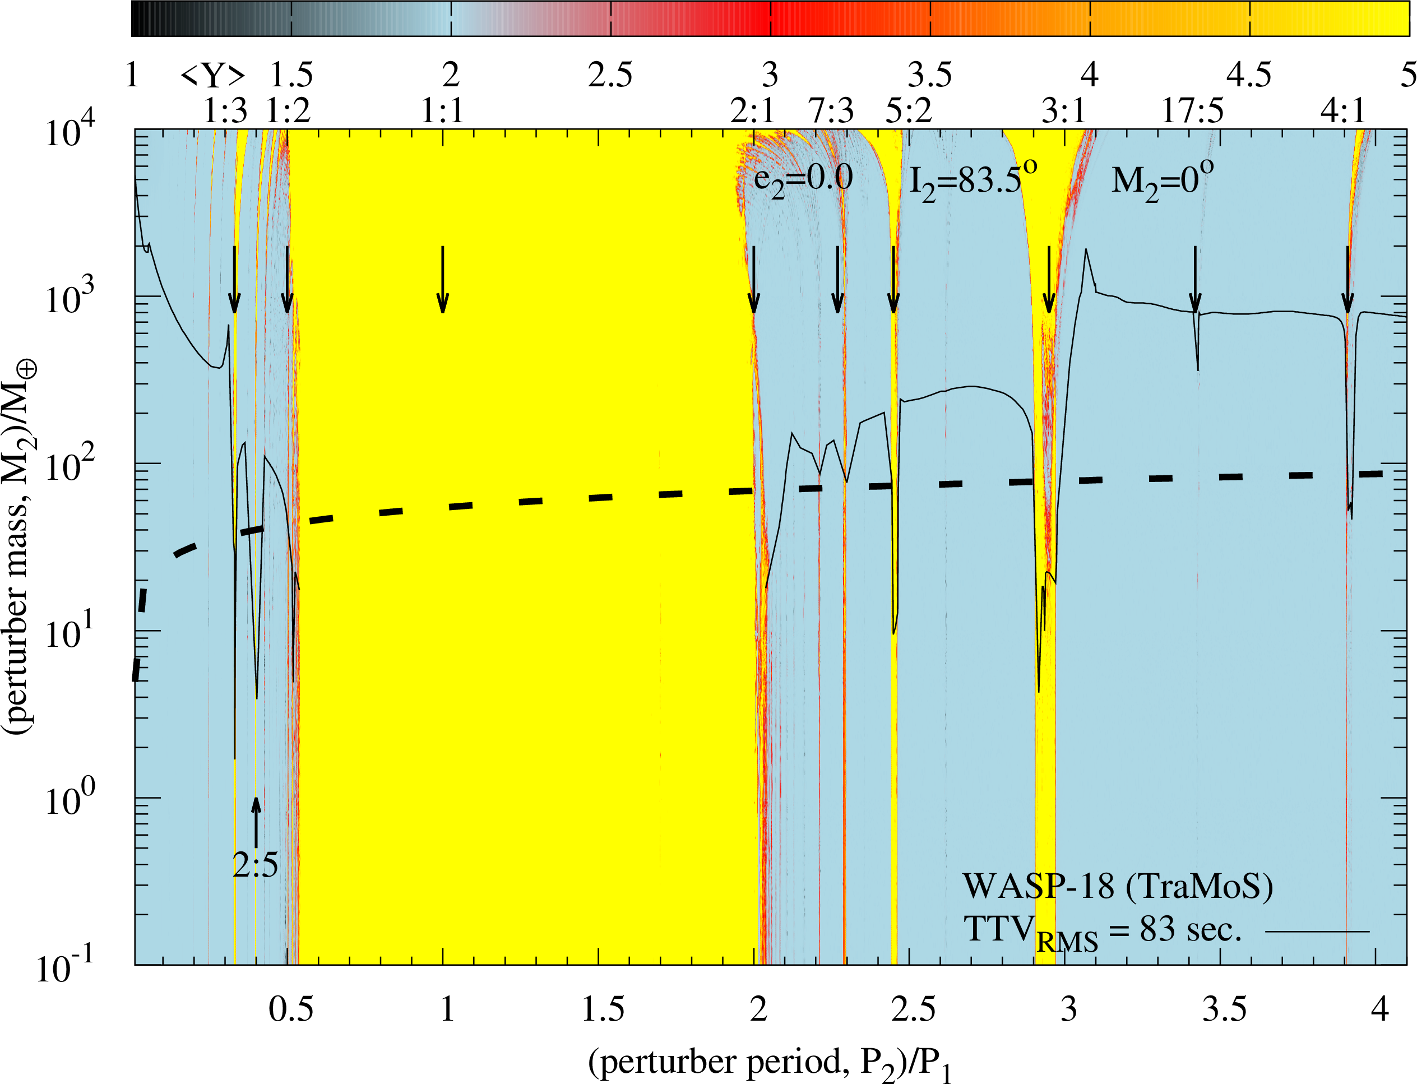
\includegraphics[width=1.0\columnwidth]{imagenes/WASP18_TraMos_83sec_Map001_GIMP_scaled.png}
\caption{MEGNO ($\langle Y \rangle$) stability map for the WASP-18 system. We over-plot the map with an upper mass of a hypothetical perturbing planet introducing a mid-transit time $\rm TTV_{\rm RMS}$ scatter of $83\,{\rm s}$ (solid line) as obtained in this study. The stipulated line is the upper mass limit as obtained from the RMS scatter $(30.9\, \rm m/s)$ of the radial-velocity curve. For initial conditions resulting in a quasi-periodic (i.e bounded) motion of the system, the $\langle Y\rangle$ value is close to 2.0 (color coded blue). For chaotic (i.e unstable) motion, the $\langle Y \rangle$ is diverging away from 2.0 (color coded red to yellow). Vertical arrows indicate $(P_2/P_1)$ orbital resonances between the perturbing body and the transiting planet. The two planets were assumed to be co-planar, and the perturbing planet's eccentricity was initially set to zero.
\emph{See electronic version for colors}.}
\label{megno_wasp18}
\end{figure}
